\section{SWOT-Analyse}

\begin{figure}[H]
\centering
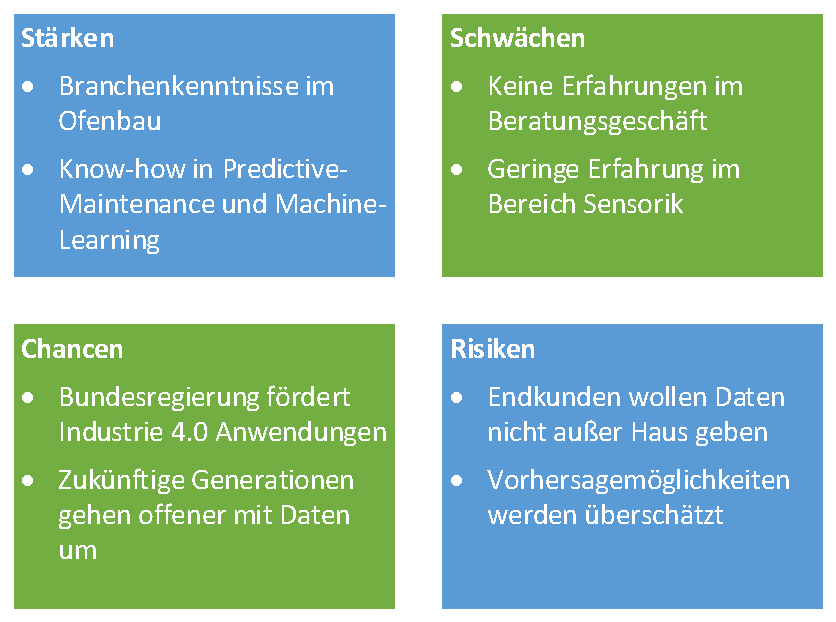
\includegraphics[width=0.7\linewidth]{Bilder/SWOT}
\caption{Unsere SWOT-Analyse}
\label{fig:SWOT}
\end{figure}


Indsutrie 4.0 ist ein Hypethema in der Wirtschaft und wird aktiv von der Bundesregierung beworben und gefördert. Wir wollen diese Chance nutzen, in dem Bereich des Atmosphärenofenbaus Predictive Maintenance als Beratungsdienstleistung anzubieten. Fehlende Erfahrung im Beratungsgeschäft und geringem Know-How im Bereich der Sensorik, stellen wir unsere langjährige Erfahrung in der Branche des Ofenbaus sowie unsere Kenntnisse im Bereich Data Analysis und Machine Learning gegenüber. Das Risiko, dass die Vorhersagemöglichkeiten unter Umständen überschätzt werden, wissen wir aufgrund unserer Erfahrung im Ofenbau und besonders im Bereich des Monitoring und Predictive Maintenance entsprechend gering einzuschätzen. Ein weiteres Risiko, dass heute Endkunden Ihre Daten gegebenenfalls nicht außer Haus geben wollen, steht der Chance gegenüber, dass zukünftige Generationen ein gänzlich anderes Verhältnis zu Daten haben und deutlich offener mit diesen umgehen werden.
